\documentclass[11pt,acticle]{scrartcl}
\usepackage{amsmath}
% \usepackage{fullpage}
\usepackage[top=1in, bottom=1in, left=0.8in, right=1in]{geometry}
\usepackage{multicol}
\usepackage{amsfonts}
\usepackage{wrapfig}
\usepackage{mathtools}
\usepackage{parskip}
\usepackage{float}
\usepackage{endnotes}


\DeclarePairedDelimiter{\ceil}{\lceil}{\rceil}
\newcommand{\overbar}[1]{\mkern 1.5mu\overline{\mkern-1.5mu#1\mkern-1.5mu}\mkern 1.5mu}
\newcommand{\R}{\mathbb{R}}
\newcommand{\N}{\mathbb{N}}
\newcommand{\Q}{\mathbb{Q}}
\newcommand{\Z}{\mathbb{Z}}
\newcommand{\C}{\mathbb{C}}
\newcommand{\ind}[1]{^{(#1)}}

\setlength{\columnsep}{1.1pc}

\title{The Perfect IHUM Essay}
\subtitle{Predicting IHUM Essay Grades}
\author{Andrew Moreland \\ Charlie Guo}
\date{}
\begin{document}
\maketitle
\rule{\linewidth}{0.4pt}

\begin{multicols}{2}

\vspace{-0.3in}
\setlength{\parskip}{10pt plus 1pt minus 1pt}

\section{Introduction}
Introduction to the Humanities -- otherwise known as IHUM -- has been a required course for Stanford freshmen for several years. IHUM is a name for a now-discontinued collection of classes that covered topics ranging from archeology and world religions to Russian literary history. Intended as a way to introduce new Stanford students to a set of core concepts in the humanities in order to assure a rounded education, IHUM has been havily criticized for its opaque and (to students) seemingly arbitrary grading.

Our project attempts to use various features of writing and diction in order to predict the final grades of essays written for IHUM classes. We draw our training and testing examples from a corpus that we have gathered from past students' essays and apply machine learning techniques in order to classify these essays into one of two categories: A or B.

\section{Background}

Automated essay scoring has been around for some time now, with approaches and use cases becoming more varied with time. Some of the original systems were developed in the 1960's, at the request of the College Board \endnote{Dikli, S. (2006). An Overview of Automated Scoring of Essays. Journal of Technology, Learning, and Assessment, 5(1).}. One of these systems, Project Essay Grader (PEG), used simple features of the written essays in order to determine a relative ``score'' (while these features were labeled ahead of time, PEG did not use machine learning to analyze the input features). While PEG was somewhat effective, its weighting of certain features allowed it to be ``tricked'' by doing things like writing longer essays. The problem was that PEG did not analyze the semantics of the essays; instead, it only analyzed the structure.

More recently, however, other systems such as Intelligent Essay Assesor (IEA), use more sophisticated techniques to predict scores. One of these techniques is Latent Semantic Analysis (LSA), ``a statistical model of word usage that permits comparisons of the semantic similarity between pieces of textual information''. Along with IEA, other programs like Criterion and E-rater used other Natural Language Processing (NLP) techniques to generate essay scores, which proved more effective than the initial LSA approach.

Our project attempts to replicate the statistical approach of PEG but also leverages a technique associated with classifying spam emails. We implement two strategies: first we compute numeric data about the structure of the essays and use an SVM to classify them, and then we use a Multinomial Naive Bayes classifier over the word frequency counts of the essays.

\section{Data Collection}
Generally machine learning projects do better if they have a larger body of training data to draw from. We figured that since nearly every student in recent years who has passed through Stanford has taken an IHUM course, it would be easy to collect a large corpus. To facilitate this we created a site (http://ihumessayproject.com/) which allowed students to easily upload their previous IHUM essays along with the grade that they received. In reality, it turns out that people are not so willing to invest the few minutes it takes to find their old essays files and upload them. As such, we received a total of 124 usable essays, which is a fair number and more than we had hoped, but is fairly small compared to the corpuses used for other efforts. \endnote{http://urd.let.rug.nl/nerbonne/papers/Santos\_et\_al-2012-grading.pdf}

\section{Pre-Processing}
In order to generate features for our SVM, we pre-processed the essays in order to extract the following data:

\begin{enumerate}
  \item Essay length
  \item Paragraph length
  \item Number of quotations
  \item Length of quotations
  \item Average word length
  \item Word frequency (using a Porter Stemmer)
  \item Part of speech frequency (using the Natural Language Toolkit for Python\footnote{http://nltk.org/})
  \item Misspelled words (words very close to words in the dictionary according to edit distance)
  \item Flesch-Kincaid Grade Level\footnote{http://www.readabilityformulas.com/flesch-grade-level-readability-formula.php}
  \item Flesch Reading Ease Scale score\footnote{https://github.com/sebbacon/pyflesch}
  \item FOG score\footnote{http://www.readabilityformulas.com/gunning-fog-readability-formula.php}

\end{enumerate}

In addition to extracting these features, we cleaned the data by removing things like stop words\footnote{http://www.lextek.com/manuals/onix/stopwords1.html} and the headers that people included in their essays.

\section{Methodology}

\subsection{Algorithm 1: SVMs}

Initially we attempted to use SVMs to classify the essays based on the computed statistics above. We used LIBSVM\endnote{Chih-Chung Chang and Chih-Jen Lin, LIBSVM: a library for support vector machines. ACM Transactions on Intelligent Systems and Technology, 2:27:1--27:27, 2011. Software available at http://www.csie.ntu.edu.tw/~cjlin/libsvm} in order to train SVMs on $70\%$ of our collected essays. We computed training accuracy on the data with linear, polynomial, radial and sigmoid based kernels with regularization. We attempted a grid search of the various parameters of these models but were never able to achieve better than $58\%$ training accuracy. For a binary classification problem where the training data is split roughly $57-43$ between the two classes this is clearly abysmal performance, so we abandoned this strategy and moved on hoping to find more success elsewhere.

\subsection{Algorithm 2: Multinomial Naive Bayes}

We decided to start with a binary classification problem. We assigned essays to two classes. Essays that were below an $A-$ became ``B'' essays, and essays that were above a $B+$ became ``A'' essays. 

Drawing inspiration from the example of spam classification, we decided to use Multinomial Naive Bayes trained over our essays in order to classify them. We split the data set into $70\%$ training and $30\%$ testing, drawing inspiration from machine learning competitions like the Netflix Challenge and used $10-$Fold Cross Validation on the rest of the data in order to maximize our training accuracy. Upon maximizing our training error, we computed our test error against the holdout set and recorded that.

Initially we tried the most naive implementation of Naive Bayes. We simply trained our classifier on the entire vocabulary found in all of the essays and then attempted to classify using the trained model. We found that we were able to achieve roughly $60\%$ accuracy with this approach, which is barely more than what would be achieved if our classifier simply guessed the most prevelant class each time. Still, since it was more accurate than guessing that we were encouraged to explore more advanced techniques.

We researched improvements to basic Naive Bayes and found that feature selection was often the most important factor in the success of the algorithm. Research indicated that one of the simplest feature selection algorithms was often helpful -- simply removing words that only appeared in a single document helped improve the overall accuracy of the classifier. With this in mind, we reran our computation and found that our training accuracy improved to roughly $64\%$ and that our vocabulary was cut from roughly $8,000$ words down to only $3,000$.

This was still fairly poor performance but the general approach seemed promising, so we decided to attempt more advanced feature selection. Research indicated that a strong metric for feature selection in text classification problems was Mutual Information\endnote{Aggarwal, Charu C., A Survey of Text Classification Algorithms, http://www.charuaggarwal.net/text-class.pdf}. Using the rainbow classifier's\endnote{McCallum, Andrew Kachites. ``Bow: A toolkit for statistical language modeling, text retrieval, classification and clustering.'' http://www.cs.cmu.edu/~mccallum/bow.  1996.} built in algorithm for mutual information computation, we initially selected the $1000$ most informative words and saw our training accuracy jump to $84\%$.

\end{multicols}

\begin{figure}[H]
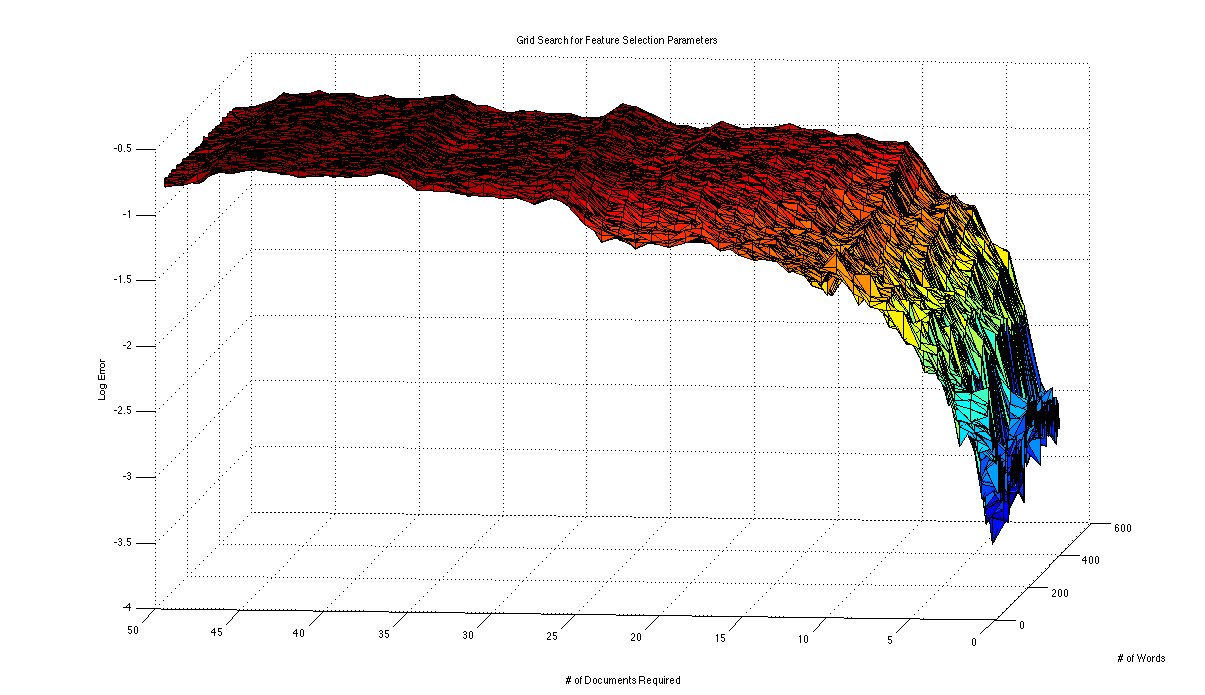
\includegraphics[scale=0.4]{feature_selection.png}
\caption{As we increased the number of documents in which a word in our vocabulary was required to appear, training accuracy sharply decreased. Our vocabulary size played a smaller and less consistent role. The error in the near right is roughly $95\%$, and the overall error moves towards $40\%$ on the left side.}
\end{figure}

\begin{multicols}{2}
At this point we decided to perform a more systematic optimization of parameters. We ran a coarse grid search over the parameter space, searching for the optimal number of documents in which to require each word to appear, and the optimal number of informative words to select as features. Our grid search ran over the integers in the intervals $[1,50]$ and $[50, 500]$ respectively. We ran a coarser grid search initially, and narrowed in on this area by an informal evaluation of the results.

Eventually, we narrowed in on a choice of the $500$ most informative words that appeared in at least $2$ documents as the optimal parameters, with which we achieved a consistent $97\%$ training accuracy. (Note: we previously observed that $500$ was a tipping point after which training accuracy decreased, so we did not evaluate anything past it in our fine grid search.)

\section{Results}
Using the parameters that we determined in our grid search, we ran tests over our $30\%$ hold out set and found that we achieved a test accuracy of $74\%$. We ran several more tests, varying the training/test size (and generating the new sets randomly each time) and found that the exact test accuracy tending to vary but was consistently over $65\%$ for reasonable training sizes. There also appears to be a trend towards convergence between test and training error somewhere between $80\%$ and $90\%$ as the training size increases.

\end{multicols}

\begin{figure}[H]
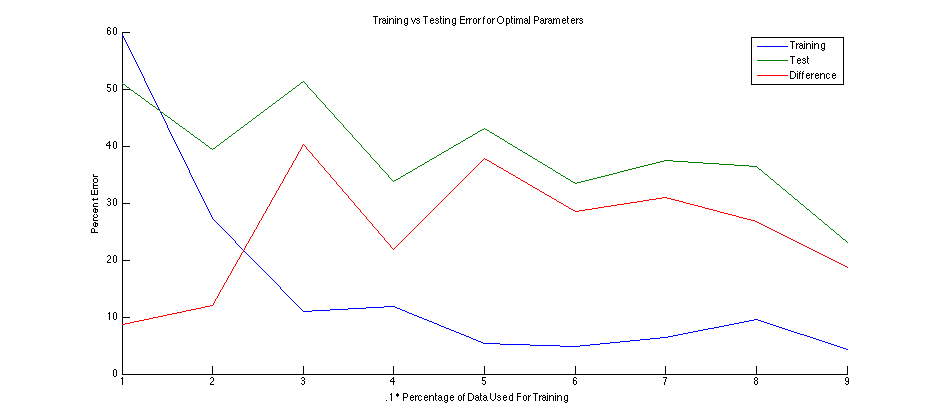
\includegraphics[scale=0.5]{error.png}
\caption{As the size of the training set increases, we see that training error tends to remain fairly constant and there appears to be a trend towards convergence.}
\end{figure}

\begin{multicols}{2}

\section{Conclusions}

Overall, we are fairly satisfied with the results of this project. We believe that we have demonstrated that it is possible to use Naive Bayes to predict a distinction between essays that is fairly fine -- the difference between an A and a B can be fairly slight.

We feel that with more training data, we could have improved the accuracy of our classifier. We feel that our results are good though given that the essays are from different eight different classes with different prompts and subjects and even more than eight graders. If we were to do the project again, we would attempt to capture more information about the context of the essays in our training set. It would have been nice to know the word limits of the essay prompts and the actual classes and graders associated with the essays. If we had known this information, then we could perhaps have applied more techniques to the data. Above all though, we express the same sentiment that many people who have attempted to apply machine learning have expressed: we wish we had more data.

\section{References}
\theendnotes
\end{multicols}
    
\end{document}
